\documentclass{article}
\usepackage{lipsum} % For placeholder text
\usepackage{listings} % For code listing
\usepackage{graphicx}
\usepackage{changepage} % Required for adjustwidth environment
\usepackage[margin=1cm]{geometry}
\usepackage{adjustbox}
\usepackage{multirow}
\usepackage{array}
\usepackage{placeins}
\usepackage{subcaption} % or \usepackage{subfigure} if using an older LaTeX distribution


\begin{document}

\title{Drought Prediction Using Various ML Algorithms}
\author{Amritesh Pandey (22-14-02)}
\date{30-05-2023}
\maketitle

\section{Introduction}

Drought is a natural disaster that severely impacts agriculture, water resources, and ecosystems. Predicting drought conditions accurately and in advance is crucial for effective resource management and mitigation strategies. Machine learning (ML) algorithms have emerged as valuable tools in drought prediction because they can analyze complex patterns and make accurate forecasts. In recent years, various ML algorithms have been applied to drought prediction with promising results. These algorithms leverage historical weather data, satellite imagery, soil moisture levels, and other relevant variables to develop models that can forecast drought conditions over specific time frames. These models can provide valuable insights into the likelihood and severity of drought, enabling stakeholders to take proactive measures to mitigate its impacts. ML algorithms offer several advantages in drought prediction. Firstly, they can handle large volumes of data and automatically identify important features and relationships, which may not be easily identifiable through traditional statistical methods. Secondly, ML algorithms can adapt and learn from new data, allowing them to continually improve their predictive capabilities. This adaptability is particularly important in drought prediction, as weather patterns and climatic conditions can change over time.

Several ML algorithms have shown promise in drought prediction. For instance, decision tree-based algorithms such as Random Forest and Gradient Boosting can capture complex interactions between weather variables and provide accurate predictions. Support Vector Machines (SVMs) can effectively handle high-dimensional data and classify drought conditions based on multiple features. Artificial Neural Networks (ANNs) can model non-linear relationships and capture intricate patterns in the data, making them suitable for drought prediction tasks. The choice of ML algorithm depends on the specific requirements of the drought prediction problem, including the available data, prediction timeframe, and desired level of accuracy. Evaluating and comparing the performance of different algorithms is essential to identify the most suitable approach for a given scenario. This can be done through metrics such as accuracy, precision, recall, and F1 score, as well as using cross-validation techniques to assess the robustness of the models.


\section{Data}

The dataset used in this study is the "US Drought Meteorological Data" dataset. It is stored in a CSV file called \texttt{train\_timeseries.csv}. The dataset contains meteorological data related to drought conditions in the United States. Each row represents a specific location identified by the \texttt{fips} code, and it includes various meteorological variables such as precipitation (\texttt{PRECTOT}), surface pressure (\texttt{PS}), specific humidity (\texttt{QV2M}), temperature (\texttt{T2M}), and wind speed (\texttt{WS10M} and \texttt{WS50M}), among others.

The dataset also includes a target variable called \texttt{score}, which represents the severity of drought at a particular location and time. The severity scores range from 0 to 5, with 0 indicating no drought and 5 indicating the most severe drought.

To load the dataset into the analysis, the \texttt{pandas} library in Python was used to read the CSV file. The dataset consists of a total of 19,300,680 entries, and it contains 21 columns in total.

The columns in the dataset represent the following variables:
\begin{itemize}
    \item \texttt{fips}: The Federal Information Processing Standards (FIPS) code that identifies a specific location.
    \item \texttt{date}: The date of the recorded meteorological data.
    \item \texttt{PRECTOT}: Total precipitation.
    \item \texttt{PS}: Surface pressure.
    \item \texttt{QV2M}: Specific humidity at 2 meters above ground level.
    \item \texttt{T2M}: Temperature at 2 meters above ground level.
    \item \texttt{T2MDEW}: Dew/frost point temperature at 2 meters above ground level.
    \item \texttt{T2MWET}: Wet bulb temperature at 2 meters above ground level.
    \item \texttt{T2M\_MAX}: Maximum temperature at 2 meters above ground level.
    \item \texttt{T2M\_MIN}: Minimum temperature at 2 meters above ground level.
    \item \texttt{T2M\_RANGE}: Temperature range at 2 meters above ground level.
    \item \texttt{TS}: Earth skin temperature.
    \item \texttt{WS10M}: Wind speed at 10 meters above ground level.
    \item \texttt{WS10M\_MAX}: Maximum wind speed at 10 meters above ground level.
    \item \texttt{WS10M\_MIN}: Minimum wind speed at 10 meters above ground level.
    \item \texttt{WS10M\_RANGE}: Wind speed range at 10 meters above ground level.
    \item \texttt{WS50M}: Wind speed at 50 meters above ground level.
    \item \texttt{WS50M\_MAX}: Maximum wind speed at 50 meters above ground level.
    \item \texttt{WS50M\_MIN}: Minimum wind speed at 50 meters above ground level.
    \item \texttt{WS50M\_RANGE}: Wind speed range at 50 meters above ground level.
    \item \texttt{score}: Drought severity score ranging from 0 to 5.
\end{itemize}

The dataset provides a valuable resource for analyzing and predicting drought conditions based on meteorological variables. By exploring and analyzing this dataset, valuable insights can be gained to improve drought management strategies and develop early warning systems.

\section{Exploratory Data Analysis (EDA)}

\subsection{Data Wrangling}

Data wrangling, also known as data preprocessing or data cleaning, is the process of transforming and preparing raw data into a format suitable for analysis. It involves handling missing values, dealing with outliers, reformatting data types, and performing any necessary transformations or adjustments.

In the code provided, the following data wrangling steps were performed:

\begin{itemize}
    \item \textbf{1. Initial Exploration and Data Cleaning:} The code initially explores the dataset by calling \texttt{drought\_df.info()} to obtain information about the data types and missing values in each column. It is observed that the \texttt{score} column has a significant number of missing values.
    
    \item \textbf{2. Missing Value Treatment:} Since the \texttt{score} column represents the target variable and is missing for most rows, it is not suitable to impute or fill the missing values. Therefore, the code drops the rows with missing values using \texttt{drought\_df.dropna()}.
    
    \item \textbf{3. Reformatting the Data:} To facilitate analysis and modeling, the code performs several reformatting steps on the dataset. It creates new columns \texttt{year}, \texttt{month}, and \texttt{day} by extracting the corresponding values from the \texttt{date} column using \texttt{pd.DatetimeIndex}. Additionally, the \texttt{score} column is rounded to the nearest integer and converted to the \texttt{int} data type.
\end{itemize}

After applying these data wrangling steps, the dataset is cleaner and ready for further analysis and modeling. The resulting dataset contains 19,300,680 entries with 23 columns, including the newly created \texttt{year}, \texttt{month}, and \texttt{day} columns.

Data wrangling is an essential step in the data analysis process as it ensures the data's quality, consistency, and suitability for analysis tasks. It helps to address any issues or inconsistencies in the data, enabling more accurate and reliable insights to be extracted from the dataset.


\subsection{Statistical Data Analysis}
Statistical Data Analysis involves applying various statistical techniques to analyze and interpret the data. It includes techniques such as univariate analysis and bivariate analysis. These techniques provide descriptive statistics, visualizations, and measures of association to understand the data's properties and relationships.

\subsubsection{Univariate Analysis}
Univariate Analysis examines one variable at a time to understand its distribution and summary statistics. It helps in identifying patterns and outliers within a single variable.

\begin{itemize}
    \item \textit{\textbf{{Discriptive Statistics}}}

            Descriptive statistics help to summarize the main properties of a dataset, providing insights into its distribution, variability, and shape. These statistics are used to describe the data in a concise and meaningful way, allowing researchers, analysts, and decision-makers to interpret and draw conclusions from the data.
            \FloatBarrier
            \begin{table}[htbp]
            \centering
            \small
            \setlength{\tabcolsep}{3pt}
            \renewcommand{\arraystretch}{1.2}
            \begin{adjustbox}{width=\textwidth}
            \begin{tabular}{|l|c|c|c|c|c|c|c|c|c|c|}
            \hline
            \textbf{Variable} & \textbf{Count} & \textbf{Mean} & \textbf{Std. Dev.} & \textbf{Min} & \textbf{25th Percentile} & \textbf{Median} & \textbf{75th Percentile} & \textbf{Max} & \textbf{Skewness} & \textbf{Kurtosis} \\ \hline
            fips & 2,756,796 & 30,670.38 & 14,979.11 & 1,001.00 & 19,044.50 & 29,260.50 & 46,007.50 & 56,043.00 & -0.077367 & -1.100136 \\ \hline
            PRECTOT & 2,756,796 & 2.71 & 6.25 & 0.00 & 0.00 & 0.19 & 2.26 & 168.69 & 4.568803 & 33.304567 \\ \hline
            PS & 2,756,796 & 96.65 & 5.44 & 66.49 & 95.83 & 98.28 & 99.94 & 103.76 & -2.132573 & 4.813301 \\ \hline
            QV2M & 2,756,796 & 7.88 & 4.72 & 0.14 & 3.81 & 6.94 & 11.45 & 22.12 & 0.526605 & -0.786067 \\ \hline
            T2M & 2,756,796 & 12.90 & 10.97 & -35.44 & 4.58 & 14.21 & 22.00 & 39.33 & -0.426059 & -0.554336 \\ \hline
            T2MDEW & 2,756,796 & 7.05 & 10.20 & -35.44 & -0.88 & 7.81 & 15.67 & 26.87 & -0.302684 & -0.733896 \\ \hline
            T2MWET & 2,756,796 & 7.09 & 10.14 & -35.46 & -0.84 & 7.81 & 15.67 & 26.87 & -0.289061 & -0.758504 \\ \hline
            T2M\_MAX & 2,756,796 & 18.77 & 11.60 & -30.03 & 10.36 & 20.62 & 27.97 & 47.75 & -0.467449 & -0.508101 \\ \hline
            T2M\_MIN & 2,756,796 & 7.52 & 10.62 & -40.85 & -0.57 & 8.26 & 16.28 & 32.28 & -0.365648 & -0.446940 \\ \hline
            T2M\_RANGE & 2,756,796 & 11.26 & 6.60 & 0.00 & 6.51 & 10.62 & 15.51 & 32.28 & 0.092413 & -0.316984 \\ \hline
            TS & 2,756,796 & 14.59 & 10.27 & -35.42 & 6.11 & 16.71 & 23.75 & 39.30 & -0.396537 & -0.535722 \\ \hline
            WS10M & 2,756,796 & 2.56 & 1.36 & 0.01 & 1.53 & 2.30 & 3.23 & 9.35 & 1.112524 & 1.419724 \\ \hline
            WS10M\_MAX & 2,756,796 & 5.20 & 1.34 & 0.57 & 0.96 & 1.66 & 2.57 & 14.62 & 0.931888 & 0.705953 \\ \hline
            WS10M\_MIN & 2,756,796 & 1.92 & 1.94 & 0.26 & 1.82 & 2.82 & 4.28 & 18.72 & 1.400951 & 3.159288 \\ \hline
            WS10M\_RANGE & 2,756,796 & 3.28 & 2.30 & 0.51 & 3.82 & 5.15 & 6.88 & 22.47 & 1.287969 & 2.084432 \\ \hline
            WS50M & 2,756,796 & 5.53 & 2.84 & 0.85 & 3.82 & 7.35 & 9.49 & 28.33 & 0.861690 & 0.819908 \\ \hline
            WS50M\_MAX & 2,756,796 & 7.83 & 2.84 & 0.00 & 5.70 & 7.35 & 9.49 & 17.78 & 0.899830 & 0.988590 \\ \hline
            WS50M\_MIN & 2,756,796 & 3.12 & 2.11 & 0.42 & 1.45 & 2.77 & 4.39 & 23.37 & 0.860444 & 0.596612 \\ \hline
            WS50M\_RANGE & 2,756,796 & 4.71 & 2.18 & 0.00 & 3.14 & 4.27 & 5.81 & 23.37 & 1.214403 & 2.205205 \\ \hline
            score & 2,756,796 & 0.82 & 0.49 & 0.00 & 0.00 & 1.00 & 1.00 & 5.00 & 1.498394 & 1.387056 \\ \hline
            year & 2,756,796 & 2007.97 & 4.90 & 2000.00 & 2004.00 & 2008.00 & 2012.00 & 2016.00 & -0.000183 & -1.208783 \\ \hline
            month & 2,756,796 & 6.53 & 3.45 & 1.00 & 4.00 & 7.00 & 10.00 & 12.00 & -0.008198 & -1.207511 \\ \hline
            day & 2,756,796 & 15.72 & 8.80 & 1.00 & 8.00 & 16.00 & 23.00 & 31.00 & 0.006969 & -1.194293 \\ \hline
            \end{tabular}
            \end{adjustbox}
            \caption{Descriptive Statistics}
            \label{tab:descriptive_statistics}
            \end{table}

            \begin{table}[htbp]
            \centering
            \label{tab:date_statistics}
            \begin{tabular}{|l|c|}
            \hline
            \textbf{Variable} & \textbf{Value} \\ \hline
            count & 2,756,796 \\
            unique & 887 \\
            top & 2000-01-04 \\
            freq & 3,108 \\ \hline
            \end{tabular}
            \caption{Descriptive Statistics of Date}
            \end{table}
            \FloatBarrier


            
   \item \textit{\textbf{{Distribution of continuous variables}}}
            \begin{figure}[htbp]
            \centering
            \begin{subfigure}{0.3\textwidth}
                \centering
                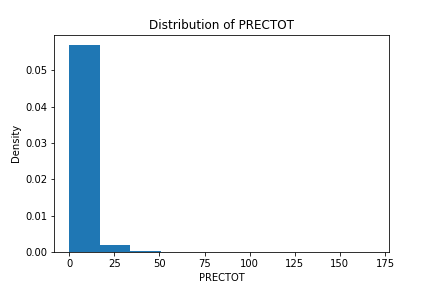
\includegraphics[width=\linewidth]{pic/hist/Distribution PRECTOT .png}
            \end{subfigure}
            \begin{subfigure}{0.3\textwidth}
                \centering
                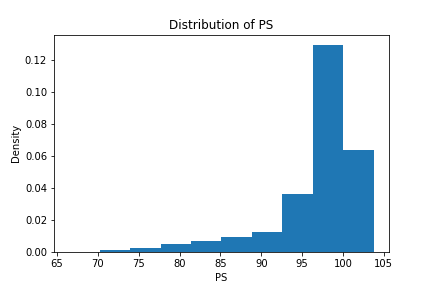
\includegraphics[width=\linewidth]{pic/hist/Distribution PS .png}
            \end{subfigure}
            \begin{subfigure}{0.3\textwidth}
                \centering
                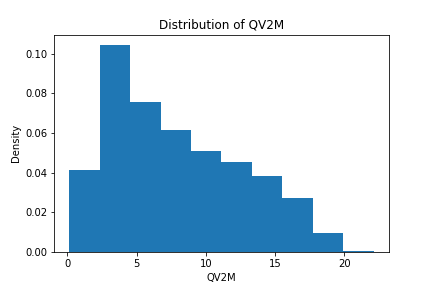
\includegraphics[width=\linewidth]{pic/hist/Distribution QV2M .png}
            \end{subfigure}
            \begin{subfigure}{0.3\textwidth}
                \centering
                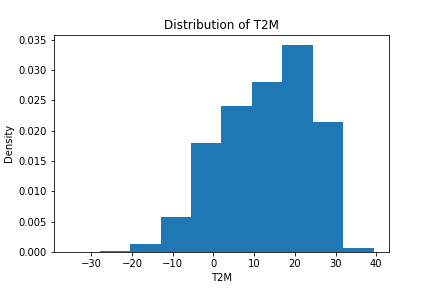
\includegraphics[width=\linewidth]{pic/hist/Distribution T2M .png}
            \end{subfigure}
            \begin{subfigure}{0.3\textwidth}
                \centering
                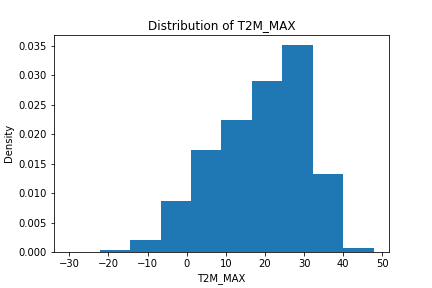
\includegraphics[width=\linewidth]{pic/hist/Distribution T2M_MAX .png}
            \end{subfigure}
            \begin{subfigure}{0.3\textwidth}
                \centering
                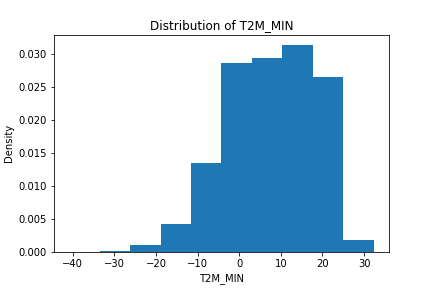
\includegraphics[width=\linewidth]{pic/hist/Distribution T2M_MIN .png}
            \end{subfigure}
            \begin{subfigure}{0.3\textwidth}
                \centering
                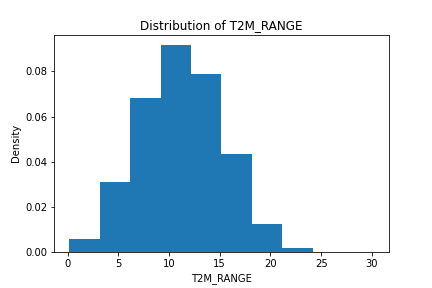
\includegraphics[width=\linewidth]{pic/hist/Distribution T2M_RANGE .png}
            \end{subfigure}
            \begin{subfigure}{0.3\textwidth}
                \centering
                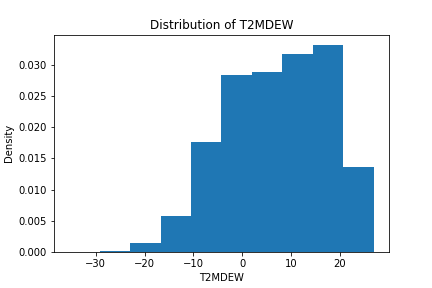
\includegraphics[width=\linewidth]{pic/hist/Distribution T2MDEW .png}
            \end{subfigure}
            \begin{subfigure}{0.3\textwidth}
                \centering
                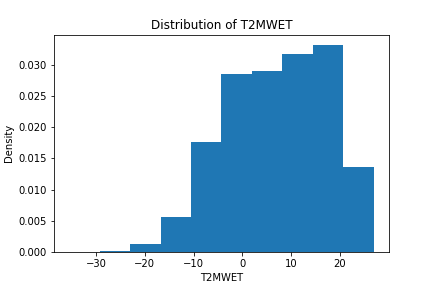
\includegraphics[width=\linewidth]{pic/hist/Distribution T2MWET .png}
            \end{subfigure}
            \begin{subfigure}{0.3\textwidth}
                \centering
                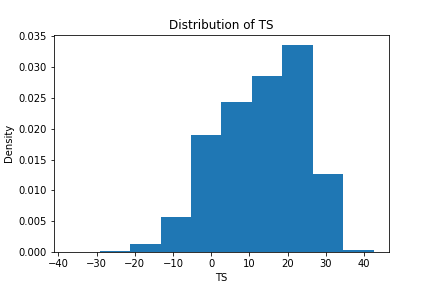
\includegraphics[width=\linewidth]{pic/hist/Distribution TS .png}
            \end{subfigure}
            \begin{subfigure}{0.3\textwidth}
                \centering
                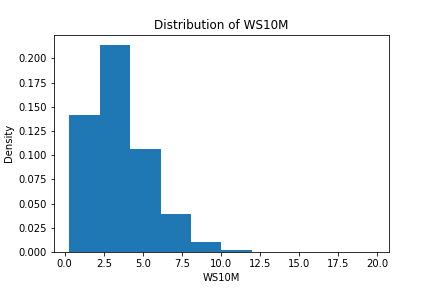
\includegraphics[width=\linewidth]{pic/hist/Distribution WS10M .png}
            \end{subfigure}
            \begin{subfigure}{0.3\textwidth}
                \centering
                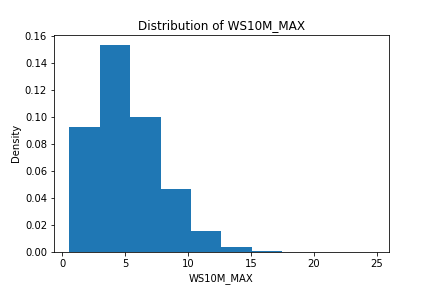
\includegraphics[width=\linewidth]{pic/hist/Distribution WS10M_MAX .png}
            \end{subfigure}
            \begin{subfigure}{0.3\textwidth}
                \centering
                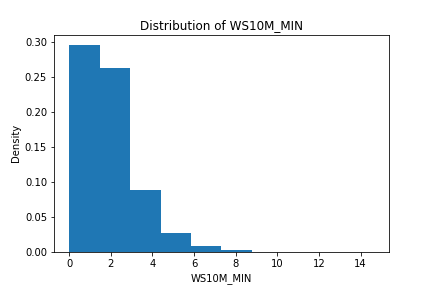
\includegraphics[width=\linewidth]{pic/hist/Distribution WS10M_MIN .png}
            \end{subfigure}
            \begin{subfigure}{0.3\textwidth}
                \centering
                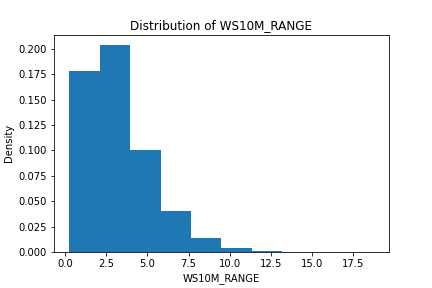
\includegraphics[width=\linewidth]{pic/hist/Distribution WS10M_RANGE .png}
            \end{subfigure}
            \begin{subfigure}{0.3\textwidth}
                \centering
                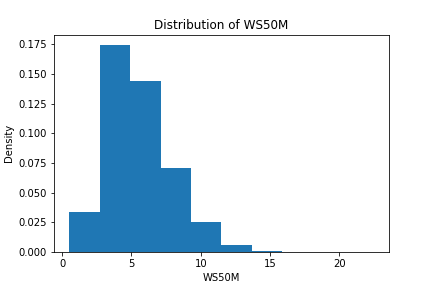
\includegraphics[width=\linewidth]{pic/hist/Distribution WS50M .png}
            \end{subfigure}
            \begin{subfigure}{0.3\textwidth}
                \centering
                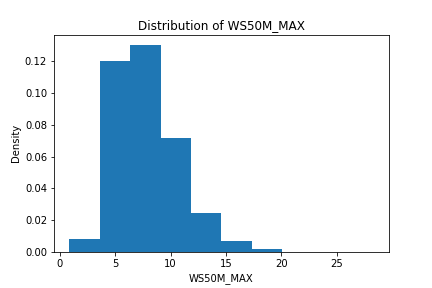
\includegraphics[width=\linewidth]{pic/hist/Distribution WS50M_MAX .png}
            \end{subfigure}
            \begin{subfigure}{0.3\textwidth}
                \centering
                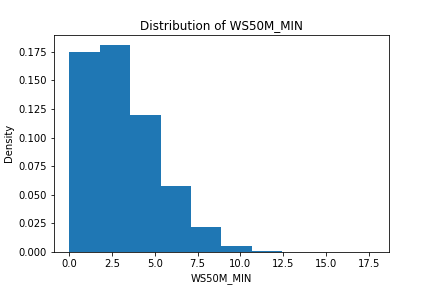
\includegraphics[width=\linewidth]{pic/hist/Distribution WS50M_MIN .png}
            \end{subfigure}
            \begin{subfigure}{0.3\textwidth}
                \centering
                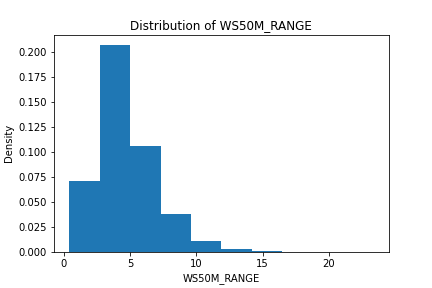
\includegraphics[width=\linewidth]{pic/hist/Distribution WS50M_RANGE .png}
            \end{subfigure}
           
            \caption{Histogram of Continuous Distribution}
            \label{fig:histogram Numerical}
            \end{figure}


           To identify outliers in continuous data, the following methods are commonly used:

                a. Summary Statistics:
                Summary statistics such as mean, median, standard deviation, and quartiles can provide insights into the central tendency and spread of the data. Unusually large or small values compared to the range of the data can be potential outliers.

                b. Box Plot:
                A box plot displays the distribution of data through quartiles, median, and outliers. Outliers are plotted as individual data points outside the whiskers of the box plot. Points outside the whiskers can be considered potential outliers.

                c. Histogram:
                A histogram represents the distribution of data by dividing it into bins and displaying the frequency or count of observations in each bin. Unusual values that fall outside the normal range of the distribution can be considered outliers.

           In the notebook provided you can see that we used histograms \ref{fig:histogram Numerical}Figure 1 and box plots to find the outliers and then removed them. 

           \item \textit{\textbf{{Distribution of categorical variables}}}

           \begin{figure}[htbp]
            \centering
            \begin{subfigure}{0.3\textwidth}
                \centering
                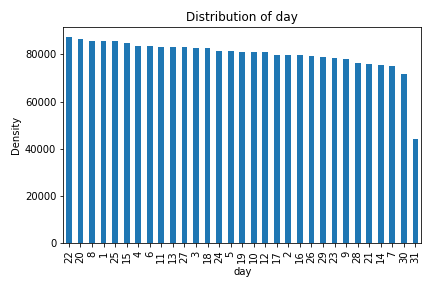
\includegraphics[width=\linewidth]{pic/hist/Distribution day.png}
            \end{subfigure}
            \begin{subfigure}{0.3\textwidth}
                \centering
                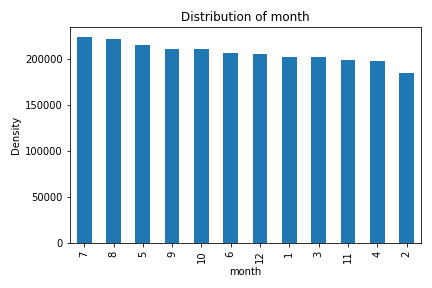
\includegraphics[width=\linewidth]{pic/hist/Distribution month.png}
            \end{subfigure}
            \begin{subfigure}{0.3\textwidth}
                \centering
                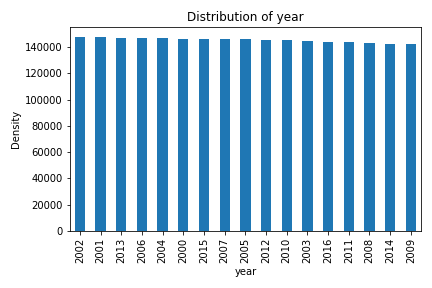
\includegraphics[width=\linewidth]{pic/hist/Distribution year.png}
            \end{subfigure}
            \begin{subfigure}{0.3\textwidth}
                \centering
                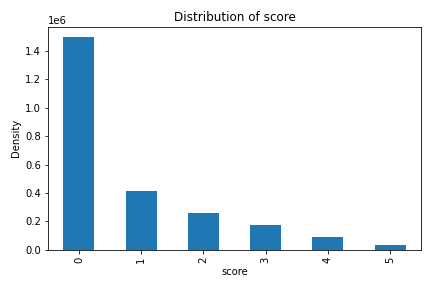
\includegraphics[width=\linewidth]{pic/hist/Distribution score.png}
            \end{subfigure}
            \caption{Histogram of Categorical Distribution}
            \label{fig:histogram Categorical}
            \end{figure}
           
           Though outliers are typically associated with continuous data, certain approaches can help identify unusual patterns or rare categories in categorical data. Here are a few methods:

                a. Frequency Histogram:
                Creating a frequency table or cross-tabulation of categorical variables allows you to observe the distribution of different categories. Categories with extremely low frequencies compared to others might be considered outliers.

                b. Bar Plot:
                Visualizing categorical variables using bar plots can help identify categories that deviate significantly from the others. If a particular category appears substantially different or unusual compared to the rest, it might be considered an outlier.

            

\end{itemize}

The following number of points were removed as they were outside the range of the outlier limit. You can check the notebook to see the boxplot which is used to visualize it:
\begin{itemize}
    \item PRECTOT -- 65933
    \item PS -- 73197
    \item QV2M -- 1
    \item T2M -- 4531
    \item T2MDEW -- 2023
    \item T2MWET -- 1814
    \item T2M\_MAX -- 3384
    \item T2M\_MIN -- 6944
    \item T2M\_RANGE -- 3628
    \item TS -- 4762
    \item WS10M -- 29954
    \item WS10M\_MAX -- 23387
    \item WS10M\_MIN -- 39901
    \item WS10M\_RANGE -- 35979
    \item WS50M -- 23090
    \item WS50M\_MAX -- 25985
    \item WS50M\_MIN -- 19569
    \item WS50M\_RANGE -- 33808
\end{itemize}
\FloatBarrier

\subsubsection{Bivariate Analysis}

Bivariate analysis is a statistical method used to analyze the relationship between two variables. It focuses on understanding how changes in one variable are related to changes in another variable. The goal is to determine if there is a correlation, association, or dependency between the two variables.

Scatterplot is used to visualize bivariate relations and these plots are shown in Figure 3

\begin{figure}[htbp]
\centering
    \begin{subfigure}{0.3\textwidth}
        \centering
        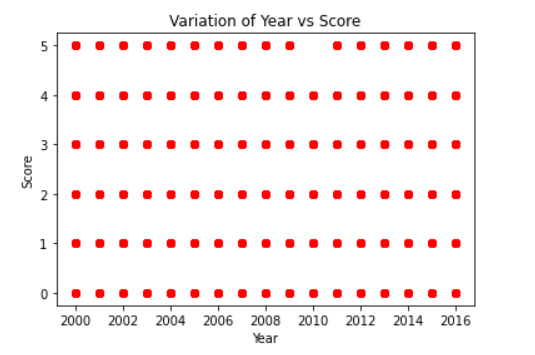
\includegraphics[width=\linewidth]{pic/scatter/Variance of Score vs Year.png}
    \end{subfigure}
    \begin{subfigure}{0.3\textwidth}
        \centering
        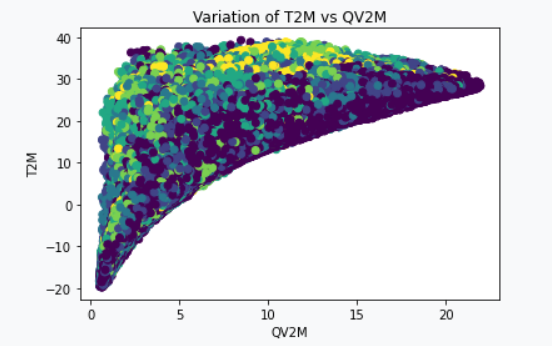
\includegraphics[width=\linewidth]{pic/scatter/Variance of T2M VS QV2M.png}
    \end{subfigure}
    \begin{subfigure}{0.3\textwidth}
        \centering
        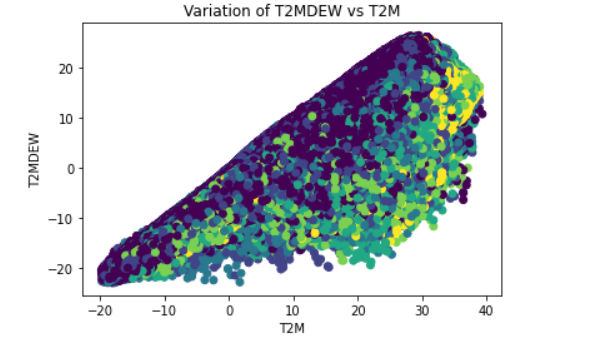
\includegraphics[width=\linewidth]{pic/scatter/VARIANCE OF T2MDEW VS T2M .png}
    \end{subfigure}
    \begin{subfigure}{0.3\textwidth}
        \centering
        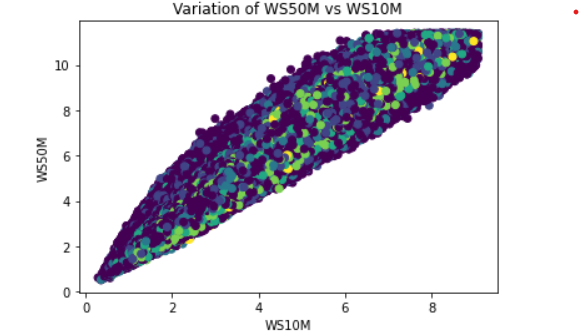
\includegraphics[width=\linewidth]{pic/scatter/VARIANCE OF WS50M VS WS10M.png}
    \end{subfigure}
\caption{Scatterplot of data}
\label{fig: Scatterplot of Data}
\end{figure}

\section{Feature Selection}

Feature selection is the process of selecting a subset of relevant features or variables from a larger set of available features in a dataset. The goal of feature selection is to identify the most informative and discriminative features that have the most impact on the target variable or outcome. By selecting the most relevant features, we can improve the performance of machine learning models by reducing overfitting, improving interpretability, and reducing computational complexity.

We first extracted the dependent variable from the data by creating another dataframe of independent variables: fips, Score, and Date.
Then we created \textbf{correlation matrix} of all the independent variables which is shown in Figure 4.

\begin{figure}[htbp]
\centering
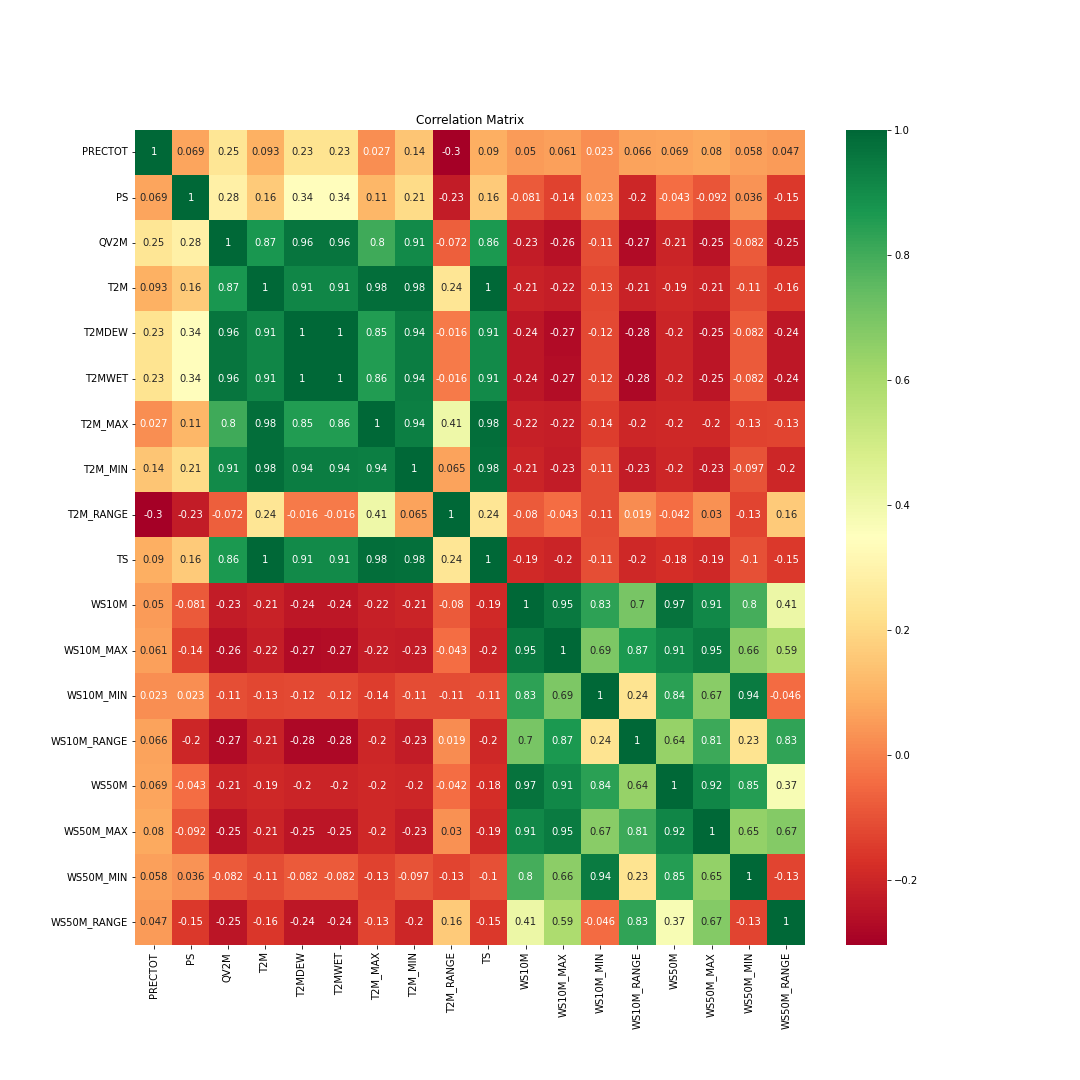
\includegraphics[width=\linewidth]{pic/correlation_plot.png}
\caption{Scatterplot of data}
\label{fig: Scatterplot of Data}
\end{figure}

\FloatBarrier


The analysis of the correlation plot reveals several strong positive correlations between different attributes in the dataset. Specifically, the attributes QV2M, T2M, T2MDEW, T2MWET, T2M\_MAX, T2M\_MIN, and TS exhibit a strong positive correlation. Similarly, the attributes WS10M, WS10M\_MAX, and WS10M\_MIN also show a strong positive correlation. Additionally, the attributes WS50M, WS50M\_MAX, and WS50M\_MIN demonstrate a strong positive correlation.

However, despite these strong positive correlations, when we examine the scatter plots of these attribute pairs, we observe significant variance among the data points. This suggests that although there is a linear relationship between these attributes, other factors might also contribute to the observed variations.

Considering the presence of significant variance, we decide to retain all these variables for further analysis and explore alternative feature selection methods. By doing so, we can capture the complex interactions and potential influences of these variables on the target variable more comprehensively.


\subsection{Feature Selection using Recursive Feature Elimination (RFE) and Random Forest Classifier}
\paragraph{Random Forest Classifier:}
Random Forest is an ensemble learning algorithm that combines multiple decision trees to make predictions. It is called "random" because each decision tree in the forest is trained on a random subset of the training data and uses a random subset of features. The predictions from all the individual trees are then aggregated to make the final prediction. Random Forests are known for their high accuracy, robustness against overfitting, and ability to handle large datasets with high dimensionality.

\paragraph{Recursive Feature Elimination (RFE):}
Recursive Feature Elimination is a feature selection technique that aims to identify the most important features in a dataset. It works by recursively eliminating less important features until a specified number of features remains. RFE assigns importance scores to each feature based on a specified model's evaluation metric (e.g., accuracy, coefficient values, etc.). It starts with all the features and ranks them based on their importance scores. Then, it recursively eliminates the least important feature(s) and re-ranks the remaining features until the desired number of features is reached.

\paragraph{Combining Random Forest Classifier with RFE:}
The Random Forest Classifier can be used as the underlying model for RFE to evaluate the importance of features. Here's how they are used together:
\begin{itemize}
    \item \textbf{Random Forest Classifier Initialization:} \\
    The code begins by initializing a Random Forest Classifier with \texttt{n\_estimators=10}. This sets up the Random Forest model with 10 decision trees. The number of estimators is a hyperparameter that determines the number of decision trees in the ensemble. 
    
    \item \textbf{RFE Initialization:} \\
    The next step is to initialize the RFE class with \texttt{n\_features\_to\_select=15}. This sets up RFE to select the top 15 features based on their importance scores. The \texttt{n\_features\_to\_select} parameter specifies the desired number of features to be selected.

    \item \textbf{Fitting RFE on the Training Data:} \\
    The code then fits the RFE model on the training data using the \texttt{fit()} method. This process involves evaluating the importance of each feature using the Random Forest Classifier. The RFE model recursively eliminates less important features and ranks the remaining features based on their importance scores.

    \item \textbf{Accessing the Selected Features:} \\
    After fitting the RFE model, the code proceeds to retrieve the selected features. The \texttt{fit.support\_} attribute returns a Boolean mask indicating which features are selected. This mask represents \texttt{True} for selected features and \texttt{False} for eliminated features. The code uses the \texttt{fit.get\_support()} method to obtain the Boolean mask.

\end{itemize}

Next, the code accesses the original feature names using \texttt{independent\_variables.columns}. By indexing the columns with the Boolean mask (\texttt{fit.get\_support()}), it selects the feature names corresponding to the \texttt{True} values, which represent the selected features.

Finally, the selected feature names are stored in the \texttt{selected\_features} variable. The columns 'PRECTOT', 'T2MWET', 'WS10M\_MAX', 'WS10M\_MIN', 'WS50M\_MIN', and 'month' are removed from the DataFrame as they were not selected. 

\subsection{Spliting data for further feature extraction and model deployment}


We then split the data with 20\% as test data and 80\% as training data using train\_test\_split and standardized the data using StandardScaler by using the Scikit-Learn library. 

The training dataset consists of 1,979,470 samples with 21 features. The shape of the training features is (1979470, 21), indicating that there are 1,979,470 rows and 21 columns in the training feature matrix. The training target variable has a shape of (1979470,), indicating that it is a 1-dimensional array with 1,979,470 elements. 

Similarly, the test dataset consists of 494,868 samples with 21 features. The shape of the test features is (494868, 21), indicating that there are 494,868 rows and 21 columns in the test feature matrix. The test target variable has a shape of (494868,), indicating that it is a 1-dimensional array with 494,868 elements. 

These shapes provide important information about the size and structure of the training and test datasets, allowing for proper data handling and analysis during the machine learning process.

\subsection{Balancing Class Imbalance by downsampling and upsampling}
Class imbalance refers to a situation in a machine learning or statistical classification problem where the distribution of classes in the training data is not equal. In other words, one class may have significantly more or fewer instances than the other class or classes. This imbalance can pose challenges for classification algorithms because they may struggle to learn patterns and make accurate predictions for the minority class.

In binary classification, class imbalance occurs when the proportion of positive examples (typically the minority class) differs significantly from the proportion of negative examples (typically the majority class). For example, in a medical diagnosis task where the goal is to detect a rare disease, the number of positive cases may be much smaller than the number of negative cases.

Similarly, in multi-class classification, class imbalance can occur when the distribution of instances across different classes is highly skewed. For instance, if you're building a model to classify images of animals, you may have significantly more images of dogs and cats than images of rare species like tigers or pandas.

The presence of class imbalance can impact the performance of classification algorithms. Since they are often designed to optimize overall accuracy, models tend to be biased towards the majority class, ignoring the minority class and leading to poor predictions for it. This is especially problematic when the minority class is the one of interest or when misclassifying the minority class has severe consequences.


\subsubsection{Upsampling}
Upsampling, also known as oversampling, involves increasing the number of instances in the minority class to balance the class distribution. This technique can be performed by duplicating existing instances from the minority class or by generating synthetic data points. Synthetic Minority Over-sampling Technique (SMOTE) is a popular algorithm used for upsampling. SMOTE creates new synthetic instances by interpolating between existing instances in the minority class, effectively increasing the representation of the minority class in the dataset.

The initial shape of the training data before oversampling is as follows:
\begin{itemize}
    \item train\_X: (1979470, 15) - This means there are 1,979,470 instances in the training set, with each instance having 15 features.
    \item train\_y: (1979470,) - This indicates that the corresponding labels for the instances in train\_X are stored in train\_y, resulting in a 1-dimensional array of length 1,979,470.
\end{itemize}

After applying SMOTE for oversampling, the shape of the training data becomes:
\begin{itemize}
    \item train\_X: (7173186, 15) - The number of instances in train\_X has increased to 7,173,186, and the number of features per instance remains the same.
    \item train\_y: (7173186,) - The length of train\_y has also increased to 7,173,186 to match the number of instances in train\_X.
\end{itemize}

The oversampling process using SMOTE has generated synthetic samples for the minority class, resulting in an increased number of instances in the training set. This approach aims to balance the class distribution and improve the performance of the classification model on the minority class.

\subsubsection{Downsampling} 
Downsampling, also known as undersampling, involves reducing the number of instances in the majority class to achieve a more balanced class distribution. This technique randomly selects a subset of instances from the majority class so that the number of instances in the majority class becomes closer to the number of instances in the minority class. By discarding some of the instances from the majority class, downsampling aims to prevent the classifier from being biased towards the majority.

The downsampling is done in two methods:

\paragraph{Neighborhood Cleaning Rule (NCR):}
     The Neighborhood Cleaning Rule is a downsampling technique that involves examining the instances in the majority class and selectively removing instances based on their proximity to instances in the minority class. Here's an overview of how NCR works:
       \begin{itemize}
            \item Identify the k nearest neighbors: For each instance in the majority class, the algorithm finds its k nearest neighbors from the minority class.
            \item Evaluate the cleanliness of neighbors: The algorithm calculates the ratio of majority class neighbors to minority class neighbors. If this ratio exceeds a specified threshold, the instance is considered "clean" and is retained. Otherwise, it is considered "unclean" and may be removed.
            \item Remove unclean instances: The unclean instances, identified based on the threshold, are removed from the majority class, resulting in a downsized dataset.
        \end{itemize}
NCR aims to preserve the instances in the majority class that are surrounded by predominantly minority class instances, while removing instances that are closer to other majority class instances.

 \paragraph{NearMiss:}
 NearMiss is another downsampling technique that focuses on selecting instances from the majority class that are close to instances in the minority class. There are several variations of NearMiss, each with a slightly different approach, but the general idea is to keep instances that are most similar to the minority class instances. Here's a general outline of the NearMiss algorithm:
        \begin{itemize}
            \item NearMiss version 1: For each instance in the minority class, the algorithm identifies the k nearest neighbors from the majority class. It selects instances from the majority class that are closest to the minority class instances based on some distance measure (e.g., Euclidean distance).
            \item NearMiss version 2 and version 3: These variations focus on selecting instances based on the average distance to the k nearest neighbors in the majority class. NearMiss version 2 selects the instances with the highest average distance, while NearMiss version 3 selects the instances with the lowest average distance.
            \item NearMiss version 3 with multiple nearest neighbors: This variation considers multiple nearest neighbors from the majority class when calculating the average distance, providing a more comprehensive representation of the neighborhood.
        \end{itemize}
NearMiss aims to retain instances from the majority class that are most similar to the minority class instances, thereby reducing the imbalance in the class distribution.

\hfill


\paragraph{Result}
The initial shape of the training data before undersampling is as follows:

\begin{itemize}
    \item train\_X: (1979470, 15) - This means there are 1,979,470 instances in the training set, with each instance having 15 features.
    \item train\_y: (1979470,) - This indicates that the corresponding labels for the instances in train\_X are stored in train\_y, resulting in a 1-dimensional array of length 1,979,470.
\end{itemize}

After applying undersampling techniques, such as Neighborhood Cleaning Rule (NCR) and NearMiss, the shape of the training data changes.


\hspace{1cm}

For Neighborhood Cleaning Rule (NCR):

\begin{itemize}
    \item train\_X: (1568791, 15) - The number of instances in train\_X has reduced to 1,568,791, while the number of features per instance remains the same.
    \item train\_y: (1568791,) - The length of train\_y has also reduced to 1,568,791 to match the number of instances in train\_X.
\end{itemize}

NCR selectively removes instances from the majority class based on their proximity to instances in the minority class. This downsampling technique aims to create a more balanced class distribution.


\hspace{1cm}

For NearMiss:

\begin{itemize}
    \item train\_X: (172842, 15) - The number of instances in train\_X has reduced to 172,842, while the number of features per instance remains the same.
    \item train\_y: (172842,) - The length of train\_y has also reduced to 172,842 to match the number of instances in train\_X.
\end{itemize}

NearMiss selects instances from the majority class that are close to instances in the minority class, thereby reducing the imbalance in the class distribution.

\subsection{Dimensionality Reduction}
Dimensionality reduction refers to the process of reducing the number of features or variables in a dataset while preserving as much relevant information as possible. It is commonly used in machine learning and data analysis to address the curse of dimensionality, improve computational efficiency, and enhance interpretability.

High-dimensional datasets with a large number of features can present several challenges. Some of these challenges include increased computational complexity, difficulty in visualizing the data, potential overfitting, and the presence of redundant or irrelevant features. Dimensionality reduction techniques aim to alleviate these challenges by reducing the number of features while retaining the most informative aspects of the data.
Here we have used two methods for dimensionality reduction:
\begin{enumerate}
    \item Principal Component Analysis
    \item Linear Discriminant Analysis
\end{enumerate}

\subsubsection{Principal Component Analysis (PCA)}
PCA is an unsupervised linear dimensionality reduction technique that aims to find a new set of orthogonal variables called principal components. It identifies the directions (principal components) along which the data varies the most. Here's an overview of how PCA works:
\begin{itemize}
    \item Data projection: PCA projects the original high-dimensional data onto a lower-dimensional subspace by linearly transforming the data.
    \item Variance maximization: PCA selects the principal components in descending order of their corresponding variances. The first principal component captures the maximum variance in the data, the second principal component captures the second highest variance orthogonal to the first, and so on.
    \item Dimension selection: The user specifies the desired number of principal components or the amount of variance to be preserved in the reduced space.
    \item Reconstruction: The reduced-dimensional data can be projected back into the original feature space, allowing for interpretation or visualization.
\end{itemize}
PCA is often used for exploratory data analysis, visualization, noise reduction, and feature compression. It is especially useful when the data has a high dimensionality and the majority of the variance is concentrated in a smaller subspace. PCA is unsupervised, meaning it does not take class labels or specific tasks into account.
Here in PCA, we used 5 principal components as it explain around 90\% of the variance in data.


\subsection{Linear Discriminant Analysis (LDA)}
LDA is a supervised dimensionality reduction technique that focuses on maximizing class separability by finding a lower-dimensional representation that maximizes the inter-class distances while minimizing the intra-class distances. LDA is commonly used for classification tasks. Here's a summary of how LDA works:
\begin{itemize}
    \item Class separability: LDA analyzes the class structure in the data by maximizing the ratio of between-class scatter to within-class scatter.
    \item Feature transformation: LDA transforms the original features into a new set of lower-dimensional features that optimally discriminate between classes.
    \item Dimension selection: The number of dimensions is usually set to the number of classes minus one, as the goal is to maximize class separability.
\end{itemize}
LDA assumes that the data follows a Gaussian distribution and that the classes have equal covariance matrices. It is effective when there is a clear separation between classes and the dimensionality reduction can enhance the classification performance.

\begin{itemize}
    \item Train features shape before LDA: (1979470, 15)
This indicates that the original training dataset had 1,979,470 instances with 15 features each.
    \item LDA Dimensionality reduced features shape on SMOTE upsampled data: (7173186, 5)
After applying LDA to the upsampled data, the dimensionality reduced features have a shape of 7,173,186 instances with 5 features each. LDA has transformed the features into a new space where the dimensionality is reduced while maximizing the class separability.
    \item LDA Dimensionality reduced features shape on the test data: (494868, 5)
The dimensionality reduction using LDA has also been applied to the test data, resulting in a shape of 494,868 instances with 5 features each.
\end{itemize}

\section{Model Deployment}
Model deployment refers to the process of making a trained machine learning model available and operational for use in a production environment. It involves taking the model that has been developed and tested during the machine learning pipeline and deploying it to a system or platform where it can be accessed and utilized to make predictions on new data.

The deployment process typically involves the following steps:
\begin{itemize}
    \item Model Export: The trained model is saved or exported in a format that can be easily loaded and utilized by the deployment environment. Common formats include serialized files or model object representations.
    \item Setting up the Deployment Environment: The deployment environment is prepared to host the model. This can involve configuring hardware resources, installing necessary software dependencies, and setting up any required infrastructure.
    \item Integration: The deployed model needs to be integrated with the existing system or application where it will be used. This may involve writing code to handle input/output interfaces, connecting to databases or data sources, and ensuring compatibility with other components.
    \item Scalability and Performance Optimization: Depending on the anticipated usage and requirements, the deployed model may need to be optimized for scalability and performance. This can involve techniques such as model parallelization, load balancing, or caching.
    \item Testing and Validation: The deployed model is thoroughly tested to ensure it functions as expected in the production environment. This includes testing the input/output interfaces, verifying the model's performance on new data, and addressing any potential issues or bugs.
    \item Monitoring and Maintenance: Once the model is deployed, it is important to monitor its performance and ensure that it continues to deliver accurate and reliable results. Regular maintenance and updates may be required to address changes in the data distribution, system updates, or evolving business requirements.
\end{itemize}
Overall, model deployment aims to make the trained model accessible and operational for real-world use, allowing it to provide predictions or decision-making capabilities in a production environment.

These are the models we deployed:
\begin{itemize}
    \item Decision Tree without resampling
    \item Decision Tree with Near Miss Downsampling
    \item Decision Tree with SMOTE Upsampling
    \item Decision Tree with Near Miss Downsampling and PCA
    \item Decision Tree with SMOTE Upsampling and PCA
    \item Decision Tree with Near Miss Downsampling and LDA
    \item Decsion Tree with SMOTE Upsampling and LDA
    \item KNN without resampling
    \item KNN with SMOTE Upsampling
    \item KNN with Near Miss Upsampling
    \item Naive Bayes without resampling
    \item Random Forest without resampling
    \item SVM with Near Miss Downsampling
\end{itemize}
\textbf{\textit{Note - 1. The hyperparameter of every model deployed is manually tuned to get the desired result by using either  RandomizedearchCV or GridSearchCV.}}\\
\textbf{\textit{Note - 2. There are some models which are left from final result as they were giving worse results.}}

\subsection{Performance Analysis}

The performance can be seen on the Table 3

\begin{table}[htbp]
\centering
\small
\setlength{\tabcolsep}{3pt}
\renewcommand{\arraystretch}{1.2}
\begin{adjustbox}{width=\textwidth}
\begin{tabular}{|c|c|c|c|c|c|}
\hline
\textbf{Algorithm} & \textbf{Accuracy} & \textbf{Precision} & \textbf{Recall} & \textbf{F1 Score} & \textbf{Cohen Kappa Score} \\ \hline
Random Forest without resampling & 0.808959 & 0.796925 & 0.808959 & 0.798690 & 0.654981 \\
KNN without resampling & 0.798651 & 0.798294 & 0.798651 & 0.798471 & 0.657498 \\
KNN with SMOTE Upsampling & 0.795267 & 0.801758 & 0.795267 & 0.798198 & 0.657827 \\
Decision Tree with SMOTE Upsampling & 0.764228 & 0.772588 & 0.764228 & 0.767987 & 0.607222 \\
Decision Tree without resampling & 0.763337 & 0.762305 & 0.763337 & 0.762809 & 0.596681 \\
Decision Tree with SMOTE Upsampling and PCA & 0.691158 & 0.721815 & 0.691158 & 0.703299 & 0.504504 \\
Decsion Tree with SMOTE Upsampling and LDA & 0.602809 & 0.674628 & 0.602809 & 0.628327 & 0.394723 \\
Naive Bayes without resampling & 0.585144 & 0.449910 & 0.585144 & 0.480441 & 0.080746 \\
SVM with Near Miss Downsampling & 0.299534 & 0.512324 & 0.299534 & 0.362867 & 0.078111 \\
KNN with Near Miss Upsampling & 0.232508 & 0.566489 & 0.232508 & 0.268879 & 0.093552 \\
Decision Tree with Near Miss Downsampling & 0.224805 & 0.543185 & 0.224805 & 0.262600 & 0.078760 \\
Decision Tree with Near Miss Downsampling and LDA & 0.204748 & 0.514249 & 0.204748 & 0.249713 & 0.057772 \\
Decision Tree with Near Miss Downsampling and PCA & 0.189016 & 0.520894 & 0.189016 & 0.224072 & 0.059722 \\
\hline
\end{tabular}
\end{adjustbox}
\caption{Performance metrics}
\label{tab:Performance metrics}
\end{table}

\section{Conclusion}
\begin{itemize}
    \item \textbf{Random Forest}: The Random Forest model without resampling achieved the highest accuracy, precision, recall, F1 score, and Cohen Kappa score among all the models. This indicates that it performed exceptionally well in predicting drought. It can be considered as a reliable and robust model for drought prediction.

    \item \textbf{Decision Tree models}: Both Decision Tree without resampling and Decision Tree with SMOTE Upsampling showed relatively high accuracy and performed well in terms of precision, recall, F1 score, and Cohen Kappa score. These models also exhibited good performance in predicting drought, although slightly lower than the Random Forest model. They can be considered as viable options for drought prediction.

    \item \textbf{KNN models}: KNN without resampling and KNN with SMOTE Upsampling showed competitive performance with high accuracy, precision, recall, F1 score, and Cohen Kappa score. These models are also effective in predicting drought conditions, particularly in scenarios with imbalanced data.

    \item \textbf{Naive Bayes}: The Naive Bayes model without resampling displayed lower accuracy and Cohen Kappa score compared to other models. It may not be the best choice for predicting drought in this case.

    \item \textbf{SVM}: The SVM model with Near Miss Downsampling showed the lowest accuracy and Cohen Kappa score among all the models. It may not be well-suited for predicting drought in this context.
\end{itemize}

\section{Refrences}
\begin{thebibliography}{9}
\bibitem{mcinerney2016}
McInerney, D., Ganguly, A. R., \& Caylor, K. (2016). Using Machine Learning to Estimate Drought Risk in the United States. \textit{Journal of Hydrometeorology}, 17(1), 195-208. \url{https://journals.ametsoc.org/doi/10.1175/JHM-D-14-0211.1}

\bibitem{nghiem2017}
Nghiem, L. X., AghaKouchak, A., Dogan, A., \& Norouzi, H. (2017). Machine learning approaches for drought prediction in the southwestern United States. \textit{Journal of Hydrology}, 549, 373-386. \url{https://www.sciencedirect.com/science/article/pii/S0022169417303771}

\bibitem{pashaee2019}
Pashaee, M., AghaKouchak, A., Mehran, A., \& Ragno, E. (2019). Drought forecasting using machine learning methods. \textit{Journal of Hydrology}, 575, 215-230. \url{https://www.sciencedirect.com/science/article/pii/S0022169419304094}

\bibitem{yu2019}
Yu, Q., Hogue, T. S., \& Vogel, R. M. (2019). Drought prediction with machine learning methods. \textit{Journal of Hydrology}, 568, 890-904. \url{https://www.sciencedirect.com/science/article/pii/S0022169419300080}

\bibitem{prudhomme2020}
Prudhomme, C., \& Crooks, S. M. (2020). Predicting droughts using machine learning and climatic indicators. \textit{Journal of Hydrology}, 590, 125395. \url{https://www.sciencedirect.com/science/article/pii/S0022169420302603}

\bibitem{distefano2020}
Di Stefano, L., Gabriele, S., Caracciolo, D., Castellani, F., \& Antonucci, V. (2020). Machine learning for drought monitoring: Data fusion of in situ and satellite products for real-time soil moisture estimation. \textit{Remote Sensing}, 12(4), 611. \url{https://www.mdpi.com/2072-4292/12/4/611}
\end{thebibliography}


\end{document}









